\section{
F Counter construction and testing process}

 The CLAS12 panel 1b detector has $62$ counters. Each counter contain one scintillation bar wrapped with aluminized Mylar film and two PMTs covered with magnetic shielding boxes. For counter assembly, each end of the scintillator is fitted with black tape (hereon referred to as "anticookie"), which masks the corners while leaving a circular window that extends one millimeter into the area that will be covered by the PMT. Apply approximately 1 $ml$ of glue to the top end of a scintillator, straight down in the center of the anticookie. Check for bubbles in glue. Since the bubbles between scintillation bars and PMTs can influence the time resolution, reapply glue to avoid bubbles. Lower the PMT in a rotating motion through the centering tools slowly onto the scintillators.

After gluing two PMTs on the end of one scintillator, the Tedlar film was wrapped the counter tightly and wrinkle-free in three layers. Retain the film
tension with electrical tape, secured only on the front side. Finish it off with a
layer of the 5-cm wide, thin, black tape running the full length of the Tedlar
sheet to avoid peeling off . Wrap 2 layers of electrical tape around PMT about $3$ cm from edge of scintillator
and at end near wires. Firmly pigtail the Tedlar film as close as reasonably possible to the PMT high voltage (HV) divider in the center with the electrical tape, trim the Tedlar to 3 cm from the
PMT HV divider, and finish the pigtail by wrapping the electrical tape around
the bundled Tedlar and cables extending to 5 cm beyond the PMT HV divider. Check that the ends closest to the PMT of the Tedlar pigtail are less than $15.5$mm in diameter in order to pass through the cable hole of the magnetic shielding box. Zip tie wires tightly using pliers at base of PMT and trim excess.

Repeat above steps for the same length six bars, then ensure that the six counters are properly aligned and secured in the six-bar rack. Connect HV, anode, and dynode cables, each set from top-left, labeled 1 to bottom-right, labeled 12. Apply baseline voltages according to PMT testing task database entries. Verify that the anode and dynode signals on the oscilloscope match the nominal documented pulse-shape distribution. Verify that the dark current is independent of light on/off status. And then start to take test run. After enough statistic data taken, the automated analysis program (section IV part G) will get the attenuation length and the time resolution of the individual counter and saved them in the database.

The backing structure is designed to support the counters in the detector space, each backing structure holds two neighbor length counters , which shows in Fig.~\ref{f:tape-rep}. There is a single-sided rubber tape between the backing structure and counters, which is in order to prevent counters to move around. Lefthanded and righthanded double-sided fiberglass tape loops, running side-by-side extending from the back corner along the back, the side, and then across the top surfaces in opposite directions, which shows in Fig.~\ref{f:tape4}, binds two counters and the backing structure tightly together. Figure~\ref{f:sector31} shows the example of double-sided fiberglass tape distribute in one backing structure precisely. Since two scintillators have different length, the close end position can only tolerate one single direction tape loop.  Then applying a single-sided, red Mylar tape loop, with both ends terminating on the back of the backing structure, to cover the double-sided fiberglass tape to avoid the peeling, which shows in Fig.~\ref{f:tape2}. After considering the room tolerance between scintillators, it is important to make sure there is no overlapping tape loop between all backing structure. The nice whole tape loop distribution for all counters is shown in Fig.~\ref{f:allsector}. Repeat above taping steps for all backing structure and assemble them as six sectors, one of them shows in Fig.~\ref{f:allsector}.

\begin{figure}[h!]
\centerline{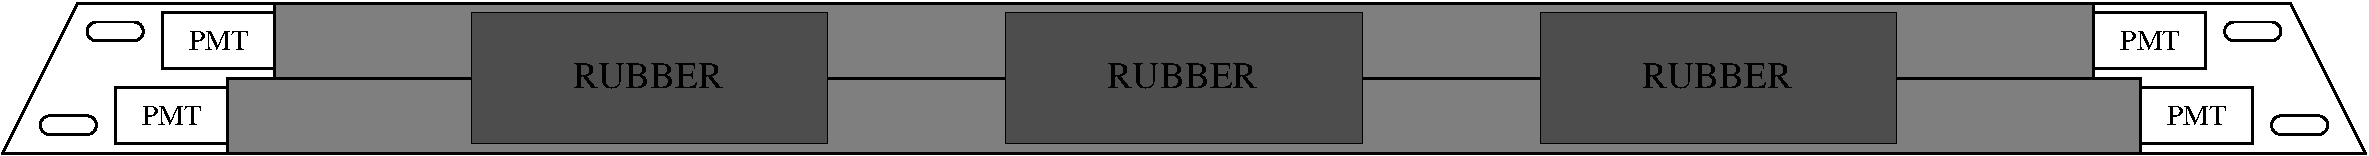
\includegraphics[width=15cm,height=1cm]{ye/fig_ye_construction/tape-replace.pdf}}
\caption{Counter structure}
\label{f:tape-rep}
\end{figure}

\begin{figure}[h!]
\begin{minipage}[h]{0.5\linewidth}
\centering
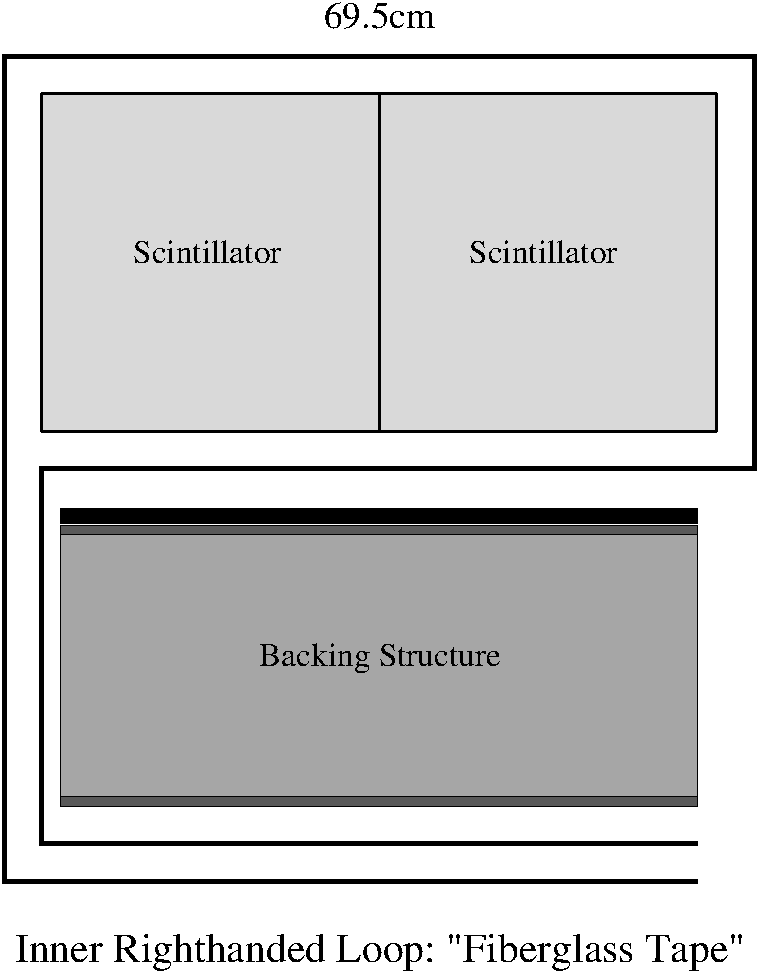
\includegraphics[width=2.0in]{ye/fig_ye_construction/fig-tape4.pdf}
\end{minipage}%
\begin{minipage}[h]{0.5\linewidth}
\centering
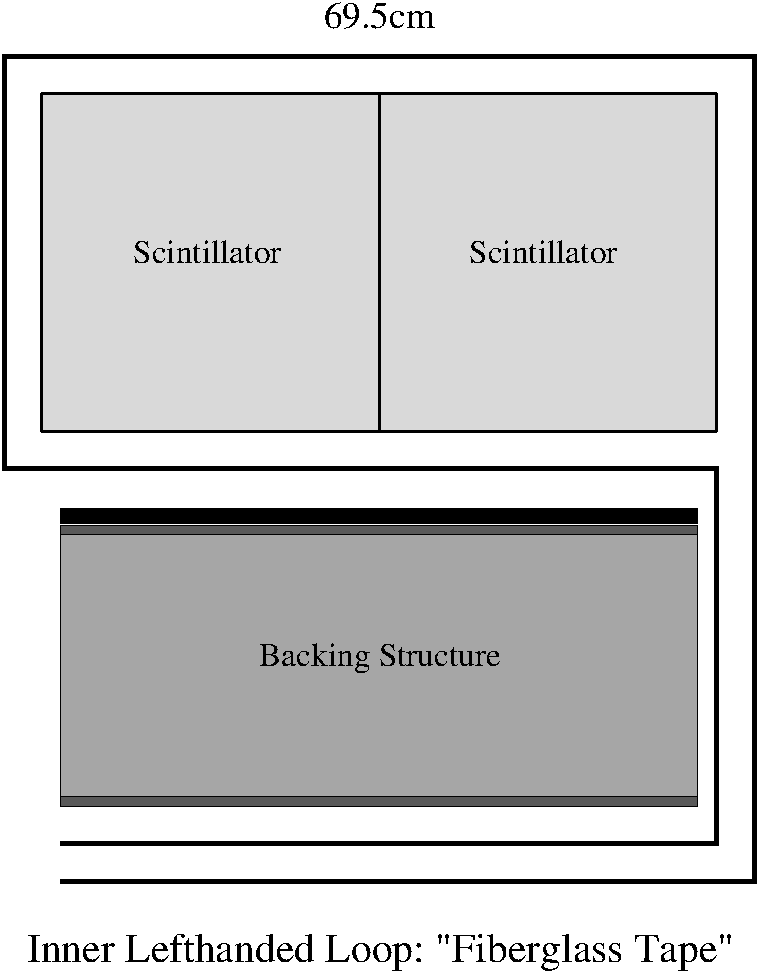
\includegraphics[width=2.0in]{ye/fig_ye_construction/fig-tape3.pdf}
\end{minipage}
\caption{Taping direction}
\label{f:tape4}
\end{figure}

\begin{figure}[h!]
\centerline{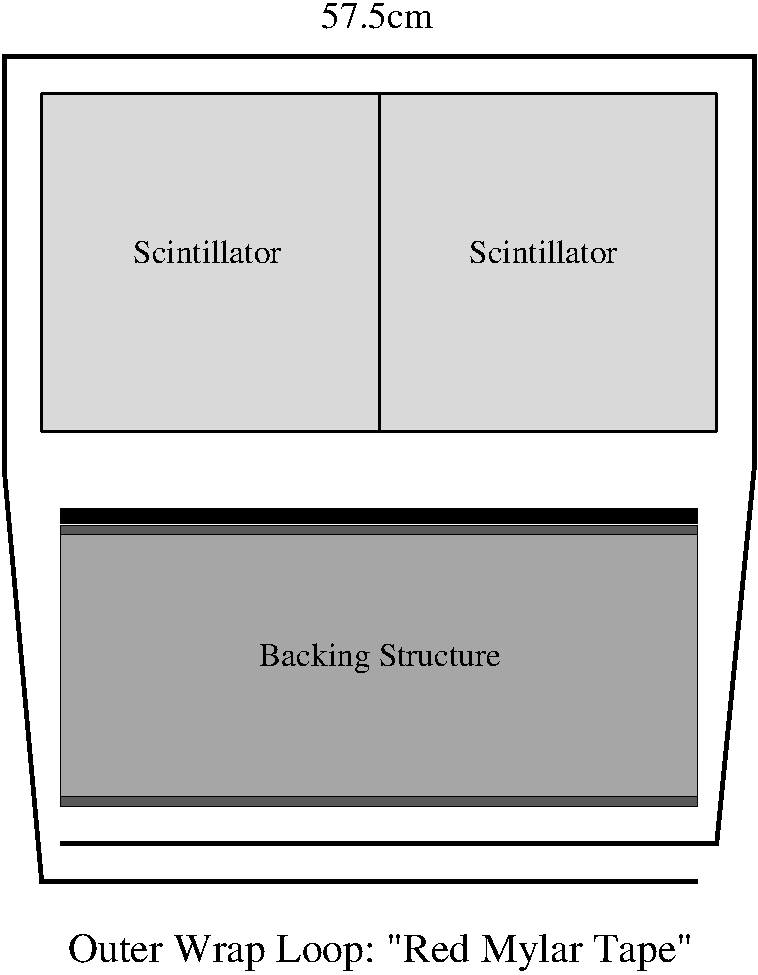
\includegraphics[width=5cm,height=7cm]{ye/fig_ye_construction/fig-tape2.pdf}}
\caption{Counter structure}
\label{f:tape2}
\end{figure}


\begin{figure}[h!]
\centerline{
\includegraphics[width=18cm,height=4cm]{ye/fig_ye_construction/sector-31-wraping.pdf}}
\caption{wrapping example of sector 31 }
\label{f:sector31}
\end{figure}
\newpage
\begin{figure}[h!]
\centerline{\includegraphics[width=18cm,height=18cm]{ye/fig_ye_construction/sector.pdf}}
\caption{Final taping structure of all sectors }
\label{f:allsector}
\end{figure}
\newpage


The following section is relate to the technical detail about PMT testing, counter assembly and testing. It can be escaped.
